% Full instructions available at:
% https://github.com/elauksap/focus-beamertheme

\documentclass[9pt]{beamer}
\usetheme{focus}

%%%%%%%%%%%%%%%%%%%%%%%%%%%%%%%%%%%%%%%%%%%%%%%%%%%%%%%%%%%%%%%%%%%%%
% Typography, change document font
\usepackage[tt=false, type1=true]{libertine}
\usepackage[varqu]{zi4}
\usepackage[libertine]{newtxmath}
\usepackage[T1]{fontenc}

\usepackage[protrusion=true,expansion=true]{microtype}

% Disable paragraph indentation, and increase gap
\usepackage{parskip}

%Matrix
\usepackage{tabstackengine}
\setstackEOL{;}% row separator
\setstackTAB{,}% column separator
\setstacktabbedgap{1ex}% inter-column gap 
\setstackgap{L}{1.0\normalbaselineskip}% inter-row baselineskip
\let\mat\bracketMatrixstack

\newcommand{\pth}{Figure/}
\newcommand{\ve}[1]{\mathbf{#1}}

% Copyright (C) 2018-2019 Pasquale Claudio Africa and the LaTeX community.
% A full list of contributors can be found at
%
%     https://github.com/elauksap/focus-beamertheme
% 
% This file is part of beamerthemefocus.
% 
% beamerthemefocus is free software: you can redistribute it and/or modify
% it under the terms of the GNU General Public License as published by
% the Free Software Foundation, either version 3 of the License, or
% (at your option) any later version.
% 
% beamerthemefocus is distributed in the hope that it will be useful,
% but WITHOUT ANY WARRANTY; without even the implied warranty of
% MERCHANTABILITY or FITNESS FOR A PARTICULAR PURPOSE. See the
% GNU General Public License for more details.
% 
% You should have received a copy of the GNU General Public License
% along with beamerthemefocus. If not, see <http://www.gnu.org/licenses/>.

\mode<presentation>


% DEFINE COLORS. ---------------------------------------------------------------
\definecolor{main}{RGB}{134, 161, 174}
\definecolor{main2}{RGB}{104, 131, 144}
\definecolor{textc}{RGB}{20, 20, 20}
\definecolor{background}{RGB}{255, 255, 255}

\definecolor{alert}{RGB}{180, 0, 0}
\definecolor{example}{RGB}{0, 110, 0}


% SET COLORS. ------------------------------------------------------------------
\setbeamercolor{normal text}{fg=textc, bg=background}
\setbeamercolor{alerted text}{fg=textc}
\setbeamercolor{example text}{fg=textc}

\setbeamercolor{titlelike}{fg=background, bg=main}
\setbeamercolor{frametitle}{parent={titlelike}}

\setbeamercolor{footline}{fg=background, bg=main2}

\setbeamercolor{block title}{bg=main!80!background, fg=background}
\setbeamercolor{block body}{bg=main!10!background, fg=textc}

\setbeamercolor{block title alerted}{bg=alert, fg=background}
\setbeamercolor{block body alerted}{bg=alert!10!background, fg=textc}

\setbeamercolor{block title example}{bg=example, fg=background}
\setbeamercolor{block body example}{bg=example!10!background, fg=textc}

\setbeamercolor{itemize item}{fg=textc}
\setbeamercolor{itemize subitem}{fg=textc}

\setbeamercolor{enumerate item}{fg=textc!70!black}
\setbeamercolor{enumerate subitem}{fg=textc!70!black}

\setbeamercolor{description item}{fg=textc!70!black}
\setbeamercolor{description subitem}{fg=textc!70!black}

\setbeamercolor{caption name}{fg=textc}

\setbeamercolor{section in toc}{fg=textc}
\setbeamercolor{subsection in toc}{fg=textc}
\setbeamercolor{section number projected}{bg=textc}
\setbeamercolor{subsection number projected}{bg=textc}

\setbeamercolor{bibliography item}{fg=main}
\setbeamercolor{bibliography entry author}{fg=main!70!black}
\setbeamercolor{bibliography entry title}{fg=main}
\setbeamercolor{bibliography entry location}{fg=main}
\setbeamercolor{bibliography entry note}{fg=main}

\mode<all>


\begin{document}
	\tableofcontents

\section{One D problem : Single variable : \today}
	\begin{frame}
		\begin{itemize}
			\item A(u(x)) = f(x) in interval 0 <x<L $\qquad$ B(u) = g
			\item Consider the differential equation
			\begin{equation}
			\begin{aligned}
				-\frac{d}{dx}\left(k(x,u) \frac{du}{dx} \right) + b(x,u)\frac{du}{dx} + c(x,u)u = f(x) \quad 0<x<L \\
				\text{Boundary conditions}\\
				n_xk\frac{du}{dx} + \beta(x,u)(u-u_{\infty}) = \hat{Q}   \quad or \quad u = \hat{u}
			\end{aligned}
			\end{equation}
			\item Note that $n_x=-1, \beta = \beta_1$ at $x = x_a$ and $n_x=1, \beta = \beta_2$ at $x = x_b$
			\item For a bar with a spring, $u_{\infty} = 0$ and we get the equation that the bar should be equal to the spring force $\beta u$. Or $-k\frac{du}{dx}-\beta_2u = Q_2 $ where Q2 is the extrenal force.
			\begin{figure}
				\centering
				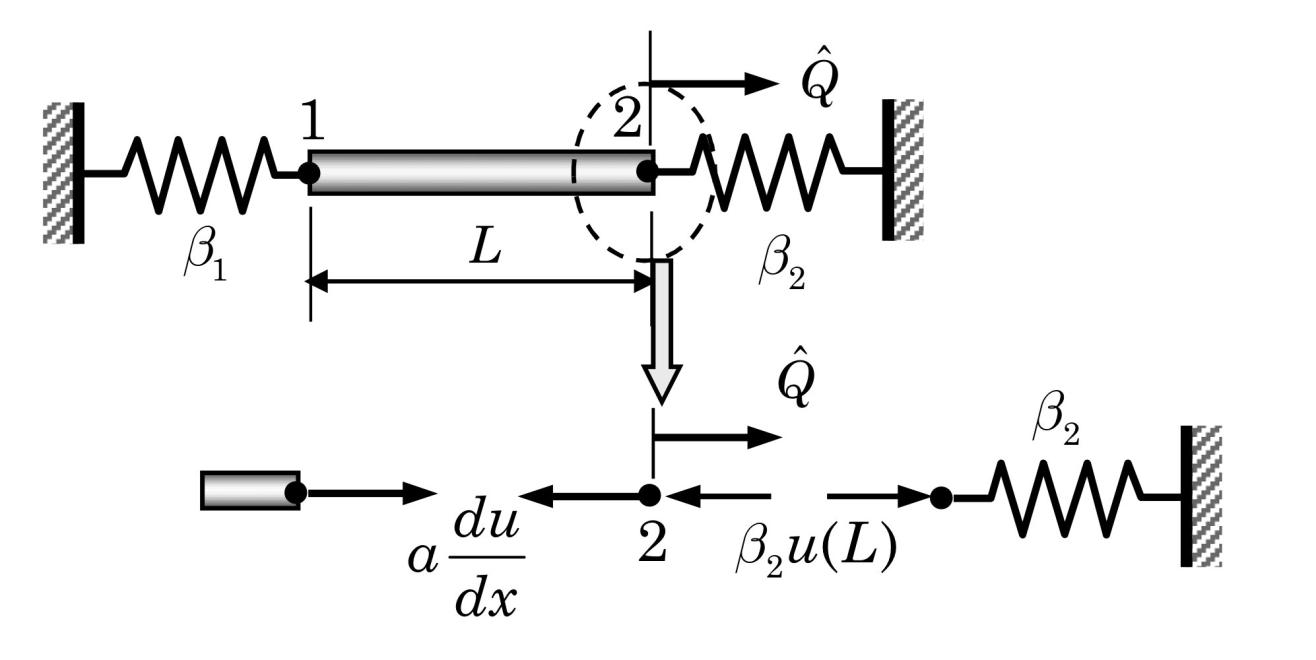
\includegraphics[width=0.7\linewidth]{Figure/fig9} 
			\end{figure} 
		\end{itemize}
	\end{frame}


	\begin{frame}
		\begin{itemize}
			\item Therefore we can keep it generally and nicely as:
			\begin{equation}
			\begin{aligned}
				A(u) = f \quad in \quad 0<x<L \qquad B(u) = g \quad at \quad x=0 or L \\
				A = -\frac{d}{dx}\left(a \frac{d}{dx} \right) +  \frac{d}{dx} + c. \quad B = n_x a \frac{d}{dx} + \beta, \quad g = \beta u_{\infty} + \hat{Q}
			\end{aligned}
			\end{equation}
			\item If a,b,c are functions of u then A and B become nonlienear.
			\item In heat a = kA, b = 0 and c = perimeter  $. \beta$
		\end{itemize}
	\end{frame}


	\begin{frame}{Weak formulation}
	\begin{figure}
			\centering
			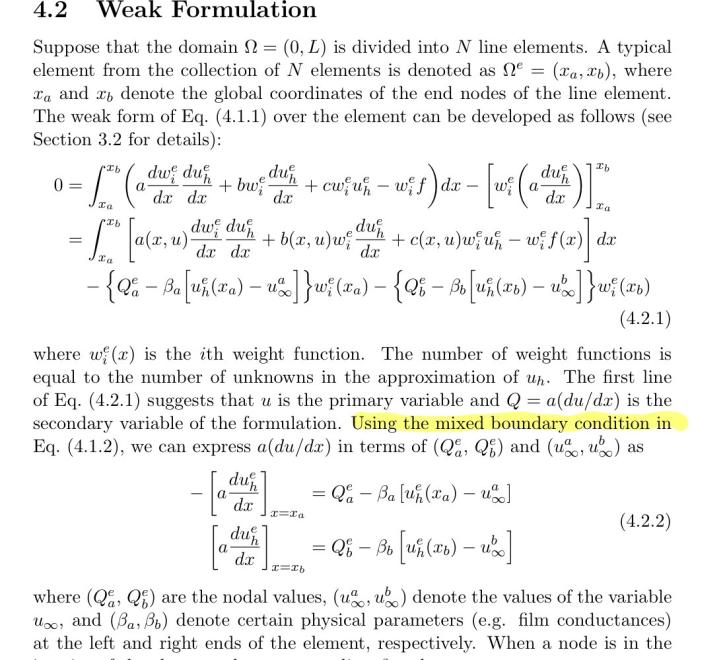
\includegraphics[width=0.7\linewidth]{Figure/fig10} 
		\end{figure}
	\end{frame}


	\begin{frame}{FEM}
		\begin{itemize}
			\item If we use the discretisation then we will get 
			\begin{equation}
			K(U)U = F
			\end{equation}
		\end{itemize} 
		\begin{figure}
		\centering
		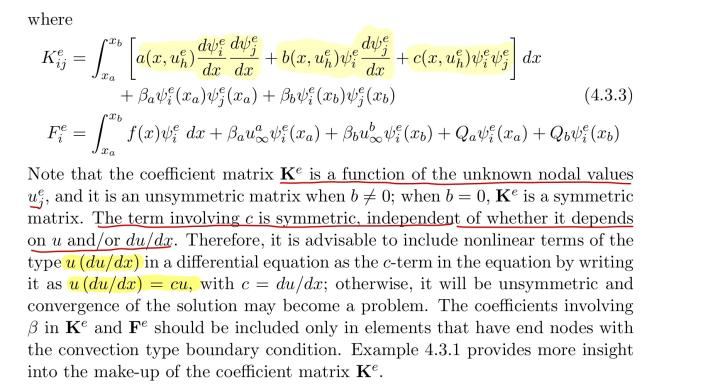
\includegraphics[width=0.8\linewidth]{Figure/fig11} 
		\end{figure}
	\end{frame}


	\begin{frame}
		\begin{itemize}
			\item The Boundary terms still confuses me. Especially the sign part. So here it is! Qe is the external force. F is the nodal force with equivalent parts. We actually get the external force from the internal Boundary terms!
			\begin{figure}
				\centering
				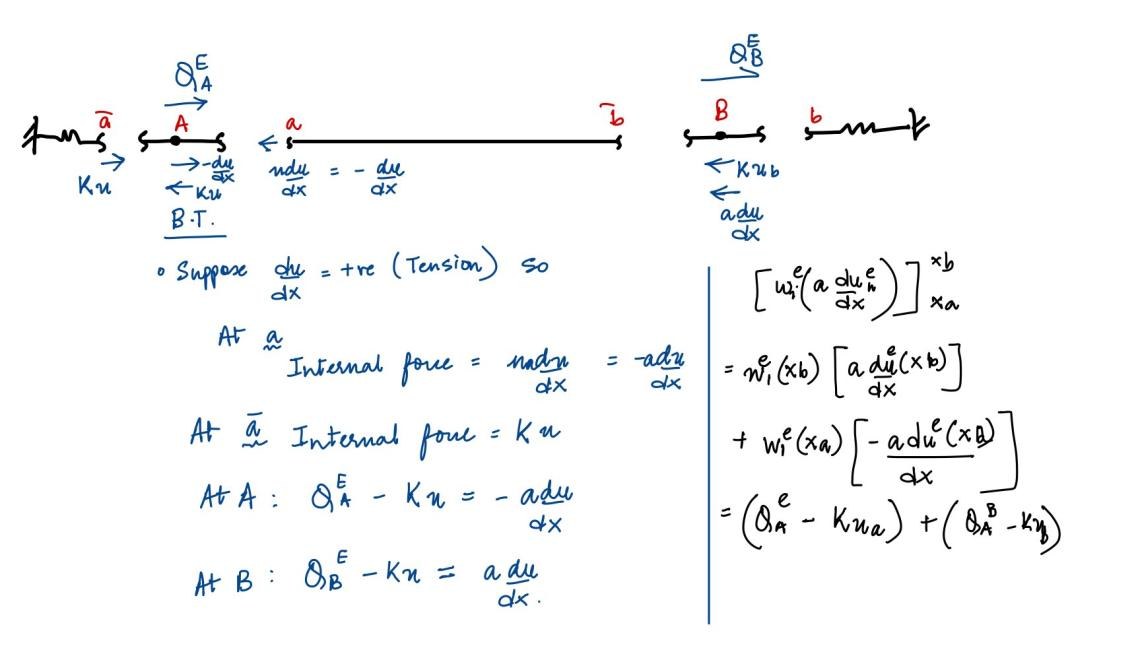
\includegraphics[width=1\linewidth]{Figure/fig12} 
			\end{figure}
			\item Check problem from Reddy for nonlinear constraints etc.
		\end{itemize}
	\end{frame}



	\begin{frame}{Solution of nonlinear algebrai equations	}
		\begin{itemize}
			\item Direct iteration procedure
			\item Newton rhapson method
		\end{itemize}
	\end{frame}


	\begin{frame}{Direct Iteration procedure}
		\begin{itemize}
			\item We solve this system of equations using direct iteration, Picard iteration or method of successive substitutions
			\begin{equation}
				\ve{K(U^{(r-1)})U^r = F(U^{(r-1)})}
			\end{equation}
			\begin{figure}
				\centering
				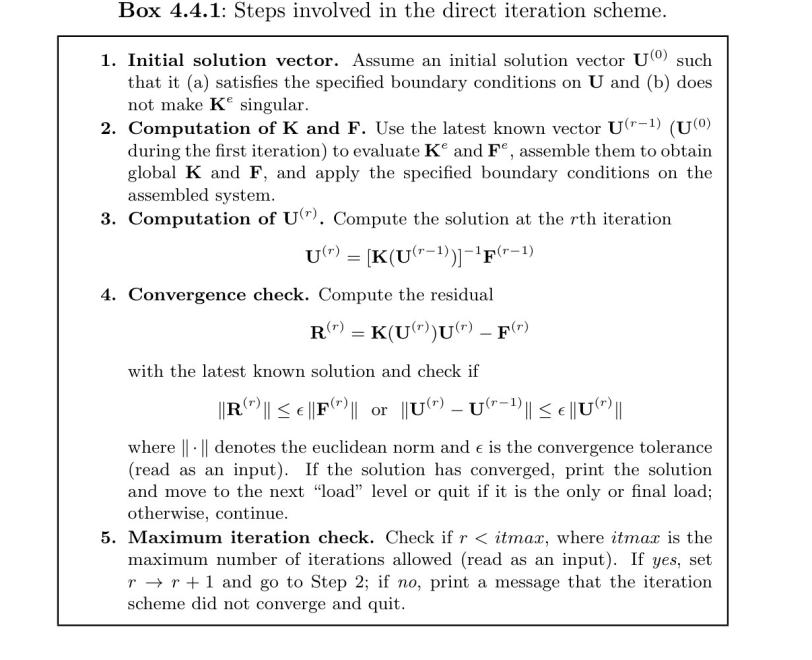
\includegraphics[width=0.8\linewidth]{Figure/fig13} 
			\end{figure}
		\end{itemize}
	\end{frame}


	\begin{frame}{Direct Iteration procedure}
		\begin{figure}
			\centering
			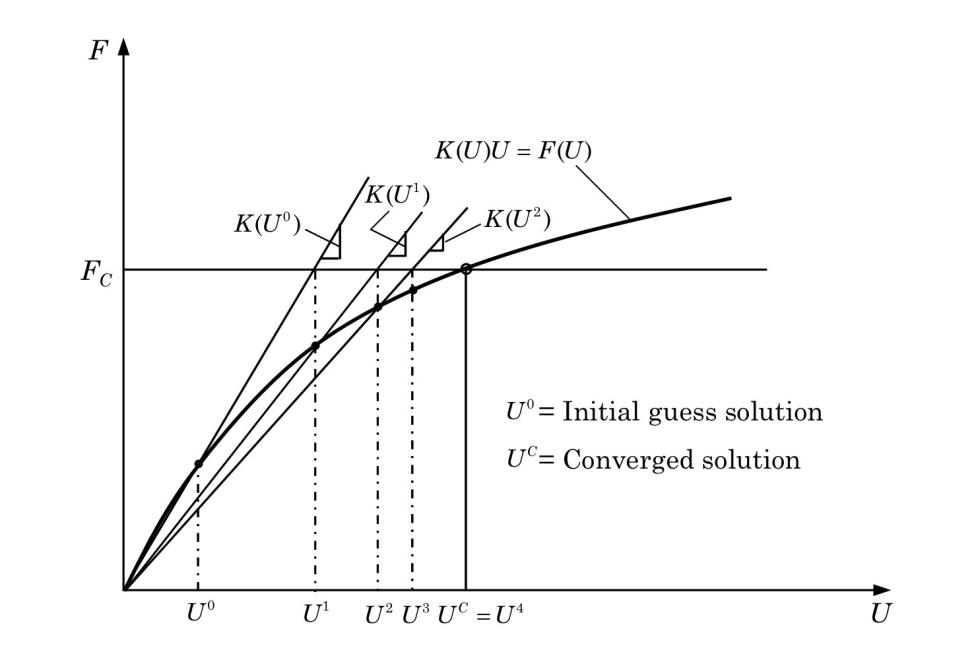
\includegraphics[width=0.5\linewidth]{Figure/fig14} 
		\end{figure}
		\begin{itemize}
			\item The method can be accelerated by using a weighted average of solutions from the last two iterations
		\begin{equation}
			\begin{aligned}
				\ve{U^r = K(\bar{U})^{-1}F(\bar{U})} \\
				\ve{\bar{U} = \beta U^{(r-2)} + (1-\beta)U^{(r-1)}}
			\end{aligned}
		\end{equation}
			\item Check Reddy 184 for some pages
		\end{itemize}
	\end{frame}


	\begin{frame}{Newtons Iteration procedure}
		\begin{itemize}
			\item In NM we expand he residual vector $\ve{R^{(r)}}$ in Taylor series about a kown solution $\ve{U^{(r-1)}}$ to get
			\begin{equation}
				\ve{R^r = R^{(r-1)} + \left(\frac{\partial R}{\partial U} \right)^{(r-1)} {\Delta} U + O(h^2)}
			\end{equation}
			where $\Delta U =  U^r - U^{(r-1)}$
			\item And saying that R in the next iteration should be zero we get
			\begin{equation}
			\begin{aligned}
				\left(\frac{\partial R}{\partial U} \right)^{(r-1)}\Delta U = -R^{(r-1)} \\
				T^{(r-1)} U^r = -R^{(r-1)}  + T^{(r-1)} U^{r-1}
			\end{aligned}
			\end{equation} 
			where T is the tangent matrix can be found at element level given as
			\begin{equation}
			\left(T_{IJ} = \frac{\partial R_I}{\partial U_J} = K_{IJ} + \sum_{m=1}^{N} \left(
			\frac{\partial K_{Im}}{\partial U_j} U_m\right) - \frac{\partial F_I}{\partial U_J} \right)^e
			\end{equation}
			The force derivative is zero if it is not a function of the load
		\end{itemize}
	\end{frame}


	\begin{frame}{NR method}
		\begin{figure}
			\centering
			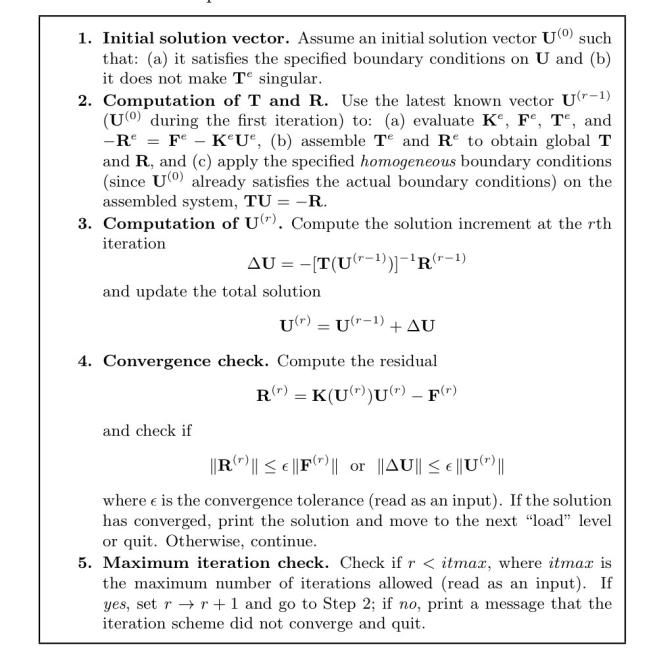
\includegraphics[width=0.5\linewidth]{Figure/fig15} 
			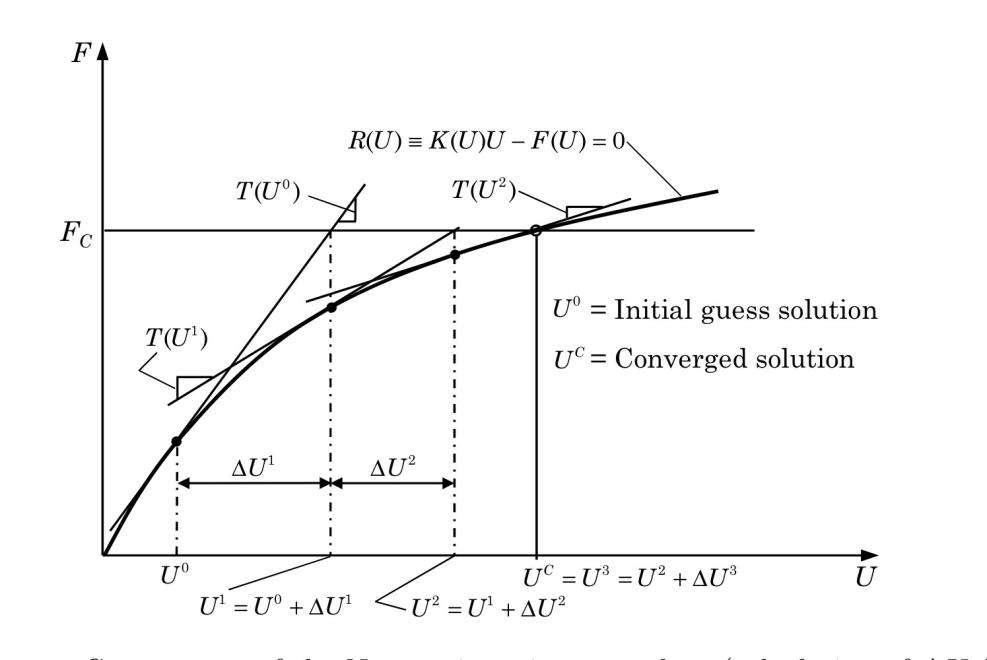
\includegraphics[width=0.45\linewidth]{Figure/fig16} 		
		\end{figure}	
	\end{frame}


	\begin{frame}{Comments}
		\begin{itemize}
			\item In the direct iteration method, the actual bc are applied at each iteration. In NR we find the increment to the known solution. If previous displ satisfies, then the increment should be zero and satisfy the boundary condition. 
			\item The symmetrry of K and T depends on the weak form. even if K is symmetric, T may not be symmetric.
			\item T can be approximate, and convergance is only when the residual is small. If it is only updated once then it is called the modified Netwons method.
			\item See the problem in Reddy -188 . Finding T	
		\end{itemize}
	\end{frame}

\end{document}
